

\chapter{Simplex Method}

\todoChapter{{\color{gray}10\% complete. Goal 80\% completion date: January 20, 2023}\\
Notes: This section hasn't been cleaned at all.  This needs to be looked at and cleaned up.}

\begin{definition}{Standard Form}{standardform}
A linear program is in \emph{standard form} if is written as 
\begin{align*}
\max \ \ &c^\top x \\
s.t. \ \ & Ax = b\\
& x \geq 0.
\end{align*}
\end{definition}

\begin{definition}{Extreme Point}{extremepoint}
A point $x$ in a convex set $C$ is called an \emph{extreme point} if it cannot be written as a strict convex combination of other points in $C$.
\end{definition}

\begin{theorem}{Optimal Extreme Point - Bounded Case}{}
Consider a linear optimization problem in standard form.  Suppose that the feasible region is bounded and non-empty. 

Then there exists an optimal solution at an extreme point of the feasible region.
\end{theorem}

\begin{proof}[Proof Sketch]

\end{proof}


% Winston
\begin{definition}{Basic solution}{}
A basic solution to $Ax = b$ is obtained by setting $n-m$ variables equal to $0$ and solving for the values of the remaining $m$ variables.  This assumes that the setting $n-m$ variables equal to 0 yields unique values for the remaining $m$ variables or, equivalently, the columns of the remaining $m$ variables are linearly independent.
\end{definition}

\begin{example}{}{}
Consider the problem
\begin{align*}
\max \quad & Z =-5 X-7 Y  \\ 
\text { s.t. } \quad & X+3 Y \geq 6 \\ 
&5 X+ 2 Y \geq 10 \\ 
&Y  \leq 4 \\ 
&X, Y  \geq 0 
\end{align*}

\begin{center}
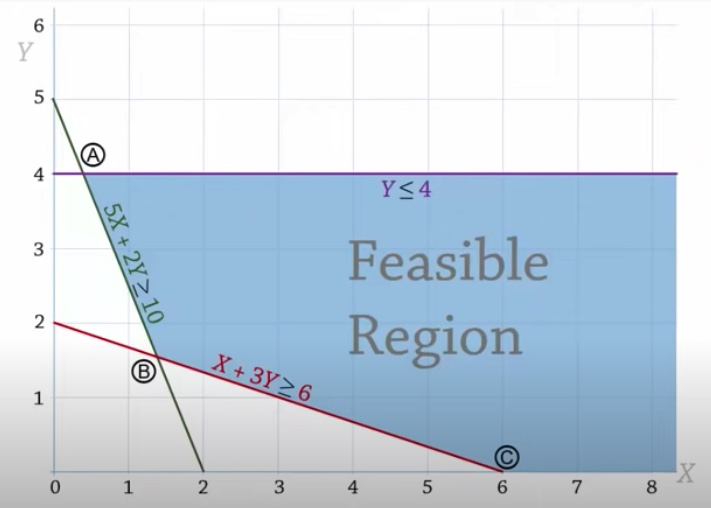
\includegraphics[scale = 0.4]{screenshots/example1-feasible-region}
\end{center}

We begin by converting this problem to standard form.  
\begin{align*}
\max \quad & Z =-5 X-7 Y + 0s_1 + 0s_2 + 0 s_3\\ 
\text { s.t. } \quad & X+3 Y - s_1 = 6 \\ 
&5 X+ 2 Y - s_2 = 10 \\ 
&Y  + s_3 = 4 \\ 
&X, Y, s_1, s_2, s_3  \geq 0 
\end{align*}

Thus, we can write this problem in matrix form with 

\begin{align}
\max  & \begin{bmatrix}
-5 \\ -7 \\ 0 \\ 0 \\0
\end{bmatrix}^\top \begin{bmatrix}
X\\Y\\s_1\\s_2\\ s_3
\end{bmatrix}\\
&\begin{bmatrix}
1 & 3 & -1 & 0 & 0 \\
5 & 2 & 0 & -1 & 0\\
0 & 1 & 0 & 0 & 1\\
\end{bmatrix}
\begin{bmatrix}
X \\ Y \\ s_1 \\ s_2 \\ s_3
\end{bmatrix}
= 
\begin{bmatrix}
6 \\ 10 \\ 4
\end{bmatrix}\\
&(X,Y,s_1, s_2, s_3) \geq 0
\end{align}


\end{example}


%Winston
\begin{definition}{Basic feasible solution}{}
Any basic solution in which all the variables are non-negative is a \emph{basic feasible solution}.
\end{definition}

%Winston
\begin{theorem}{BFS iff extreme}{}
A point in the feasible region of an LP is an extreme point if and only if it is a basic feasible solution to the LP.
\end{theorem}

To prove this theorem, we 

%Winston
\begin{theorem}{Representation}{}
Consider an LP in standard form, having bfs $b_1, \dots, b_k$.  Any point $x$ in the LP's feasible region may be written in the form 
$$
x = d + \sum_{i=1}^k \sigma_i b_i
$$
where $d$ is $0$ or a direction of unboundedness and $\sum_{i=1}^k \sigma_i = 1$ and $\sigma_i \geq 0$.
\end{theorem}

% Winston
\begin{theorem}{Optimal bfs}{}
If an LP has an optimal solution, then it has an optimal bfs.
\end{theorem}

\begin{proof}
Let $x$ be an optimal solution.  Then 
$$
x = d + \sum_{i=1}^k \sigma_i b_i
$$
where $d$ is 0 or a direction of unboundeness.  

\begin{itemize}
\item If $c^\top d > 0$, the $x'  = \lambda d + \sum_{i=1}^k \sigma_i b_i$ has bigger objective value for $|lambda > 1$, which is a contradiction since $x$ was optimal. 
\item If $c^\top d < 0$, the $x'' =\sum_{i=1}^k \sigma_i b_i$ has a bigger objective value, which is a contradiction since $x$ was optimal.
\end{itemize}
Thus, we conclude that $c^\top d = 0$.

Since $$c^\top x \geq c^\top b_i$$ for all $i=1, \dots, k$, we can conclude that 
$$
c^\top x = c^\top b_i
$$
for all $i$ such that $\sigma_i > 0$.   Hence, there exists an optimal basic feasible solution.
\end{proof}

\section{Simplex Method}

\section{Finding Feasible Basis}

\underline{\bf Finding an Initial BFS}
When a basic feasible solution is not apparent, we an produce one using {\it artificial variables}.  This {\it artificial} basis is undesirable from the perspective of the original problem, we do not want the artificial variables in our solution, so we penalize them in the objective function, and allow the simplex algorithm to drive them to zero (if possible) and out of the basis.  There are two such methods, the {\bf Big M method} and the {\bf Two-phase method}, which we illustrate below:

\vspace{10mm}  Solve the following LP using the Big M Method and the simplex algorithm:

\begin{align*}
max~~ & z = 9x_1 + 6x_2 \\
s.t.~~
&  3x_1 + 3x_2 \le 9 \\
&  2x_1 - 2x_2 \ge 3 \\
&  2x_1 + 2x_2 \ge 4 \\
& x_1, x_2 \ge 0. \\
\end{align*}

Here is the LP is transformed into standard form by using slack variables $x_3$, $x_4$, and $x_5$, with the required artificial variables $x_6$ and $x_7$, which allow us to easily find an initial basic feasible solution (to the artificial problem).
\begin{eqnarray}
& max  & z_a = 9x_1 + 6x_2 -M x_6 - M x_7 \nonumber \\
& s.t. & 3x_1 + 3x_2 + x_3 = 9 \nonumber \\
&      & 2x_1 - 2x_2 - x_4 + x_6 = 3 \nonumber \\
&      & 2x_1 + 2x_2 - x_5 + x_7 = 4 \nonumber \\
&      & x_i \ge 0,~~ i =1,\cdots,7. \nonumber
\end{eqnarray}

\begin{center} \begin{tabular} {|c|c|c|c|c|c|c|c||c| r} \cline{1-9}
$z$	& $x_1$	& $x_2$	& $x_3$	& $x_4$	& $x_5$	& $x_6$	& $x_7$	& RHS &	ratio \\ \cline{1-9}
1	&	 -9 &	 -6 &	 0 &	  0 &	  0 &	  M &	  M &	0 & \\
0	&	  3 &	  3 &	 1 &	  0 &	  0 &	  0 &	  0 &	9 &	 \\
0	&	  2 &	 -2 &	 0 &	 -1 &	  0 &	  1 &	  0 &	3 & \\
0	&	  2 &	  2 &	 0 &	  0 &	 -1 &	  0 &	  1 &	4 &	 \\
\cline{1-9}
\end{tabular} \end{center}
\noindent This tableau is not in the correct form, it does not represent a basis, the columns for the artificial variables need to be adjusted.

\begin{center} \begin{tabular} {|c|c|c|c|c|c|c|c||c| r} \cline{1-9}
$z$	& $x_1$	  & $x_2$  & $x_3$	& $x_4$	& $x_5$	& $x_6$	& $x_7$	& RHS &	ratio \\ \cline{1-9}
1	& -9 - 4M & -6     &	 0 &	  M &	  M &	  0 &	  0 & -7M &	      \\
0	&	  3   &	     3 &	 1 &	  0 &	  0 &	  0 &	  0 &	9 &	3     \\
0	&	  2   &	    -2 &	 0 &	 -1 &	  0 &	  1 &	  0 &	3 &	3/2   \\
0	&	  2   &	     2 &	 0 &	  0 &	 -1 &	  0 &	  1 &	4 &	2     \\
\cline{1-9}
\end{tabular} \end{center}
\noindent The current solution is not optimal, so $x_1$ enters the basis, and by the ratio test, $x_6$ (an artificial variable) leaves the basis.

\begin{center} \begin{tabular} {|c|c|c|c|c|c|c|c||c| r} \cline{1-9}
$z$	&   $x_1$ & $x_2$   & $x_3$	& $x_4$	& $x_5$	& $x_6$	   & $x_7$	& RHS      & ratio \\
\cline{1-9}
1	&     0   & -15 -4M &	 0 & -9/2 -M &	  M & 9/2 + 2M &	  0 &  27/2 -M &    	\\
0	&	  0   &	     6  &	 1 &	 3/2 &	  0 &	    -3/2 &	  0 &	3/2    & 3/4     \\
0	&	  1   &	    -1  &	 0 &	-1/2 &	  0 &	   1/2 &	  0 &	3/2    & -  	\\
0	&	  0   &	     4  &	 0 &	   1 &	 -1 &	     -1 &	  1 &	  1    & 1/4        	\\ \cline{1-9}
\end{tabular} \end{center}
\noindent The current solution is not optimal, so $x_2$ enters the basis, and by the ratio test, $x_7$ (an artificial variable) leaves the basis.

\begin{center} \begin{tabular} {|c|c|c|c|c|c|c|c||c|r} \cline{1-9}
$z$	&   $x_1$ & $x_2$ & $x_3$ & $x_4$	& $x_5$	& $x_6$	   & $x_7$	& RHS     &	ratio \\
\cline{1-9}
1	&     0   &     0 &	 0    & -3/4    & -15/4 &        - &	  - &  17 1/4 &	   \\
0	&	  0   &	    0 &	 1    &	   0    &	3/2 &	     0 &   -3/2 &	  3   &	-  \\
0	&	  1   &	    0 &	 0    &	-1/4    &  -1/4 &	   1/2 &	1/4 &	  7/4 &	-  	\\
0	&	  0   &	    1 &	 0    &	 1/4    &  -1/4 &	  -1/4 &	1/4 &	  1/4 & 1   \\
\cline{1-9}
\end{tabular} \end{center}
\noindent The current solution is not optimal, so $x_4$ enters the basis, and by the ratio test, $x_2$ leaves the basis.

\begin{center} \begin{tabular} {|c|c|c|c|c|c|c|c||c|r} \cline{1-9}
$z$	&   $x_1$ & $x_2$ & $x_3$ & $x_4$ & $x_5$ & $x_6$ & $x_7$ & RHS     &	ratio \\
\cline{1-9}
1	&     0   &    3  &	 0    & 0     & -9/2  &     - &	    - &  18 &	   \\
0	&	  0   &	    0 &	 1    &	   0  &	  3/2 &	    0 &  -3/2 &	  3     &	-  \\
0	&	  1   &	    1 &	 0    &	0     &  -1/2 &	   0  &	  1/2 &	  2   &	-  	\\
0	&	  0   &	    4 &	 0    &	 1    &  -1   &	  -1 &      1 &	  1    & 1   \\ \cline{1-9}
\end{tabular} \end{center}
\noindent The current solution is not optimal, so $x_5$ enters the basis, and by the ratio test, $x_3$ leaves the basis.

\begin{center} \begin{tabular} {|c|c|c|c|c|c|c|c||c|r} \cline{1-9}
$z$	&   $x_1$ & $x_2$ & $x_3$ & $x_4$ & $x_5$ & $x_6$ & $x_7$ & RHS     &	ratio \\
\cline{1-9}
1	&     0   &    3  &	 3    & 0     & 0  &     - &	    - &  27 &	   \\
0	&	  0   &	    0 &	 2/3  &	  0   &	  1 &	    0 &  -1 &	  2     &	 \\
0	&	  1   &	    1 &	 1/3   &   0  &  0 &	   0  &	  0 &	  3   &  	\\
0	&	  0   &	    4 &	 2/3   &	1 &  0   &	  -1 &     0&	 3    &    \\
\cline{1-9}
\end{tabular} \end{center}
The current solution is optimal! \\

\bigskip Solve the following LP using the Two-phase Method and Simplex Algorithm.
\begin{align*}
max~~ & z = 2x_1 + 3x_2   \\
s.t.~~ 
& 3x_1 + 3x_2 \ge 6  \\
& 2x_1 - 2x_2 \le 2  \\
& -3x_1 + 3x_2 \le 6   \\
& x_1, x_2 \ge 0. 
\end{align*}


%\begin{center} \includegraphics[scale=0.7]{Figs_N/TwoPhase}\end{center}

Here is first phase LP (in standard form), where $x_3$, $x_4$, and $x_5$ are slack variables, and $x_6$ is an artificial variable.
\begin{eqnarray}
& min  & z_a = x_6 \nonumber \\
& s.t. & 3x_1 + 3x_2 - x_3 +x_6 = 6 \nonumber \\
&      & 2x_1 - 2x_2 + x_4 = 2 \nonumber \\
&      & -3x_1 + 3x_2 + x_5 = 6 \nonumber \\
&      & x_i \ge 0,~~ i =1,\cdots,6. \nonumber
\end{eqnarray}
Next, we put the LP into a tableau, which, still is not in the right form for our basic variables ($x_6$, $x_4$, and $x_5$).
\begin{center} \begin{tabular} {|c|c|c|c|c|c|c||c| r} \cline{1-8}
$z$	& $x_1$	& $x_2$	& $x_3$	& $x_4$	& $x_5$	& $x_6$	&  RHS & ratio \\ \cline{1-8}
1	&	  0 &	  0 &	 0 &	  0 &	  0 &	 -1 &    0 & \\
0	&	  3 &	  3 &	-1 &	  0 &	  0 &	  1 &	 6 & \\
0	&	  2 &	 -2 &	 0 &	  1 &	  0 &	  0 &	 2 & \\
0	&	  -3 &	  3 &	 0 &	  0 &	  1 &	  0 &	 6 & \\ \cline{1-8}
\end{tabular} \end{center}
To remedy this, we use row operation to modify the row 0 coefficients, yielding the following:
\begin{center} \begin{tabular} {|c|c|c|c|c|c|c||c| r} \cline{1-8}
$z$	& $x_1$	& $x_2$	& $x_3$	& $x_4$	& $x_5$	& $x_6$	&  RHS & ratio \\ \cline{1-8}
1	&	  3 &	  3 &	 -1 &	  0 &	  0 &	  0 &    6 &   \\
0	&	  3 &	  3 &	-1 &	  0 &	  0 &	  1 &	 6 &  2 \\
0	&	  2 &	 -2 &	 0 &	  1 &	  0 &	  0 &	 2 &  - \\
0	&	  -3 &	  3 &	 0 &	  0 &	  1 &	  0 &	 6 &  2 \\ \cline{1-8}
\end{tabular} \end{center}
The current solution is not optimal, either $x_1$ or $x_2$ can enter the basis, let's choose $x_2$. Then by the ratio test, either $x_6$ (an artificial variable) or $x_5$ (a slack variable) can leaves the basis.  Let's choose $x_6$.
\begin{center} \begin{tabular} {|c|c|c|c|c|c|c||c| r} \cline{1-8}
$z$	& $x_1$	& $x_2$	& $x_3$	& $x_4$	& $x_5$	& $x_6$	&  RHS & ratio \\ \cline{1-8}
1	&	  0 &	  0 &	 0 &	  0 &	  0 &  -1 &    0 & \\
0	&	  1 &	  1 &	-1/3 &	  0 &	  0 &   1/3 &	 2 & \\
0	&	  4 &	  0 &	-2/3 &	  1 &	  0 &   2/3 &	 6 & \\
0	&	 -6 &	  0 &	 1 &	  0 &	  1 &	 -1 &	 0 & \\ \cline{1-8}
\end{tabular} \end{center}
The current solution is optimal, so we end the first phase with a basic feasible solution to the original problem, with $x_2$, $x_4$, and $x_5$ as the basic variables.  Now we provide a new row zero that corresponds to the original problem.

\begin{center} \begin{tabular} {|c|c|c|c|c|c|c||c| r} \cline{1-8}
$z$	& $x_1$	& $x_2$	& $x_3$	& $x_4$	& $x_5$	& $x_6$	&  RHS & ratio \\ \cline{1-8}
1	&	  1 &	  0 &	 -1 &	  0 &	  0 &	  0 &   6 & \\
0	&	  1 &	  1 &	-1/3 &	  0 &	  0 &	  1/3 &	 2 &   \\
0	&	  4 &	  0 &	-2/3 &	  1 &	  0 &	  2/3 &	 6 &  \\
0	&	 -6 &	  0 &	 1 &	  0 &	  1 &	  -1 &	 0 &  \\ \cline{1-8}
\end{tabular} \end{center}

\begin{center} \begin{tabular} {|c|c|c|c|c|c|c||c| r} \cline{1-8}
$z$	& $x_1$	& $x_2$	& $x_3$	& $x_4$	& $x_5$	& $x_6$	&  RHS & ratio \\ \cline{1-8}
1	&	 -5 &	  0 &	  0 &	  0 &	  1 &	  -1 &   6 & \\
0	&	 -1 &	  1 &	  0 &	  0 &	1/3 &	  0 &	 2 &   \\
0	&	  0 &	  0 &	  0 &	  1 &	2/3 &	  0 &	 6 &  \\
0	&	 -6 &	  0 &	  1 &	  0 &	  1 &	  -1 &	 0 &  \\ \cline{1-8}
\end{tabular} \end{center}
From this tableau we can see that the LP is unbounded and an extreme point is [0, 2, 0, 6,0] and an extreme direction is [1, 1, 6, 0, 0].




\underline{\bf Degeneracy and the Simplex Algorithm}
\begin{comment}
$\mathbf {n} \cdot (\mathbf {r} -\mathbf {r} _{0})=0.$
(The dot here means a dot (scalar) product.) Expanded this becomes

$a(x-x_{0})+b(y-y_{0})+c(z-z_{0})=0$
which is the point-normal form of the equation of a plane.  This is just a linear equation

$ax+by+cz+d=0$,
where

$d=-(ax_{0}+by_{0}+cz_{0}).$  
Conversely, it is easily shown that if a, b, c and d are constants and a, b, and c are not all zero, then the graph of the equation

$ax+by+cz+d=0$ is a plane having the vector 

$\mathbf{ n} = (a, b, c)$ as a normal. 

This plane can also be described by the "point and a normal vector" prescription above. A suitable normal vector is given by the cross product
${\mathbf {n}}=({\mathbf {p}}_{2}-{\mathbf {p}}_{1})\times ({\mathbf {p}}_{3}-{\mathbf {p}}_{1})$,

and the point r0 can be taken to be any of the given points p1,p2 or p3[6] (or any other point in the plane).
Let p1=(x1, y1, z1), p2=(x2, y2, z2), and p3=(x3, y3, z3) be non-collinear points.

${\displaystyle \mathbf {w\times v} ={\begin{vmatrix}\mathbf {i} &\mathbf {j} &\mathbf {k} \\w_{1}&w_{2}&w_{3}\\v_{1}&v_{2}&v_{3}\\\end{vmatrix}}}$

${\displaystyle {\begin{aligned}\mathbf {w\times v} &={\begin{vmatrix}w_{2}&w_{3}\\v_{2}&v_{3}\end{vmatrix}}\mathbf {i} -{\begin{vmatrix}w_{1}&w_{3}\\v_{1}&v_{3}\end{vmatrix}}\mathbf {j} +{\begin{vmatrix}w_{1}&w_{2}\\v_{1}&v_{2}\end{vmatrix}}\mathbf {k} \\&=(w_{2}v_{3}-w_{3}v_{2})\mathbf {i} +(w_{3}v_{1}-w_{1}v_{3})\mathbf {j} +(w_{1}v_{2}-w_{2}v_{1})\mathbf {k} ,\end{aligned}}}$
\end{comment}

Degeneracy must be considered in the simplex algorithm, as it causes some trouble.  For instance, it might mislead us into thinking there are multiple optimal solutions, or provide faulty insight.  Further, the algorithm as described can {\it cycle}, that is, remain on a degenerate extreme point repeatedly cycling through a subset of bases that represent that point, never leaving. 

\begin{center} \begin{tabular} {c|c|c|c|c|c|c|c|c|c|} \cline{2-10}
min &$z$	& $x_1$ & $x_2$ & $x_3$	& $x_4$	&  $x_5 $& $x_6$ & $x_7$ & $rhs$ \\ \cline{2-10}
       &1		& 0 		  & 0         &	 0 	    &	  3/4     &   -20 & 1/2 & -6  &     0    \\ \cline{2-10}
       &0		&	 1       &	    0   &	 0 			&	  1/4 		&	-8 & -1 &   9 &   0	  \\
       &0		&	 0     &	    1      &	 0 		&	  1 /2		&	 -12 & -1/2 & 3 & 0   \\ 
       &0		&	 0     &	    0      &	 1 		&	  0		&	 0 & 1 & 0 &1   \\ \cline{2-10}
\end{tabular} \end{center}


\bigskip  Solve the following LP using the Simplex Algorithm:
\begin{eqnarray}
& \max  & z = 40x_1 + 30x_2 \nonumber \\
& s.t. & 6x_1 + 4x_2 \le 40 \nonumber \\
&      & 4x_1 + 2x_2 \le 20 \nonumber \\
&      & x_1, x_2 \ge 0. \nonumber
\end{eqnarray}

By adding slack variables, we have the following tableau.
\begin{table}[h!] \begin{center} \begin{tabular} {|c|c|c|c|c||c|}
\hline
$z$ & $x_1$ & $x_2$ & $s_1$ & $s_2$ & RHS \\ \hline
  1 & -40 & -30 & 0   & 0   & 0  \\
  0 &   6 &   4 & 1   & 0   & 40 \\
  0 &   4 &   2 & 0   & 1   & 20 \\ \hline
\end{tabular} \end{center} \end{table}
Luckily, this tableau represents a basis, where BV=$\{s_1, s_2\}$, but by inspecting the row 0 (objective function row) coefficients, we can see that this is not optimal. By Dantzig's Rule, we enter $x_1$ into the basis, and by the ratio test we see that $s_2$ leaves the basis.  By performing elementary row operations, we obtain the following tableau for
the new basis BV=$\{s_1, x_1\}$.
\begin{center} \begin{tabular} {|c|c|c|c|c||c|} \hline
$z$ & $x_1$ & $x_2$ & $s_1$ & $s_2$ & RHS \\
\hline
  1 &     0 &   -10 & 0     &    10 & 200 \\
  0 &     0 &     1 & 1     &  -3/2 & 10 \\
  0 &     1 &   1/2 & 0     &   1/4 &  5 \\
\hline
\end{tabular} \end{center}

This tableau is not optimal, entering $x_2$ into the basis can improve the objective function value. The basic variables $s_1$ and $x_1$ tie in the ration test.  If we have $x_1$ leave the basis, we get the following tableau (BV=$\{s_1, x_2\}$).
\begin{center} \begin{tabular} {|c|c|c|c|c||c|}
\hline
$z$ & $x_1$ & $x_2$ & $s_1$ & $s_2$ & RHS \\
\hline
  1 &    20 &     0 &     0 &    15 & 300 \\
  0 &    -2 &     0 &     1 &    -2 &  0 \\
  0 &     2 &     1 &     0 &   1/2 &  10 \\ \hline
\end{tabular} \end{center}
This is an optimal tableau, with an objective function value of 300,  If instead of $x_1$ leaving the basis, suppose $s_1$ left, this would lead to the following tableau (BV=$\{x_2, x_1\}$).
\begin{center} \begin{tabular} {|c|c|c|c|c||c|} \hline
$z$ & $x_1$ & $x_2$ & $s_1$ & $s_2$ & RHS \\
\hline
  1 &     0 &     0 &    10 &    -5 & 300 \\
  0 &     0 &     1 &     1 &  -3/2 &  10 \\
  0 &     1 &     0 &  -1/2 &     1 &   0 \\ \hline
\end{tabular} \end{center}
This tableau does not look optimal, yet the objective function value is the same as the optimal solution's. This occurs because the optimal extreme point is a degenerate.% as the following figure shows.

